% !TEX encoding = UTF-8 Unicode
\documentclass[a4paper]{article}

\usepackage{color}
\usepackage{url}
\usepackage[T2A]{fontenc} % enable Cyrillic fonts
\usepackage[utf8]{inputenc} % make weird characters work
\usepackage{graphicx}

\usepackage[english,serbian]{babel}
%\usepackage[english,serbianc]{babel} %ukljuciti babel sa ovim opcijama, umesto gornjim, ukoliko se koristi cirilica

\usepackage[unicode]{hyperref}
\hypersetup{colorlinks,citecolor=green,filecolor=green,linkcolor=blue,urlcolor=blue}

\usepackage{listings}
\usepackage{verbatimbox,lipsum}

\usepackage{xurl}

%\newtheorem{primer}{Пример}[section] %ćirilični primer
\newtheorem{primer}{Primer}[section]

\definecolor{mygreen}{rgb}{0,0.6,0}
\definecolor{mygray}{rgb}{0.5,0.5,0.5}
\definecolor{mymauve}{rgb}{0.58,0,0.82}

\lstset{ 
  backgroundcolor=\color{white},   % choose the background color; you must add \usepackage{color} or \usepackage{xcolor}; should come as last argument
  basicstyle=\scriptsize\ttfamily,        % the size of the fonts that are used for the code
  breakatwhitespace=false,         % sets if automatic breaks should only happen at whitespace
  breaklines=true,                 % sets automatic line breaking
  captionpos=b,                    % sets the caption-position to bottom
  commentstyle=\color{mygreen},    % comment style
  deletekeywords={...},            % if you want to delete keywords from the given language
  escapeinside={\%*}{*)},          % if you want to add LaTeX within your code
  extendedchars=true,              % lets you use non-ASCII characters; for 8-bits encodings only, does not work with UTF-8
  firstnumber=1   ,                % start line enumeration with line 1000
  frame=single,	                   % adds a frame around the code
  keepspaces=true,                 % keeps spaces in text, useful for keeping indentation of code (possibly needs columns=flexible)
  keywordstyle=\color{black},       % keyword style
  language=Python,                 % the language of the code
  morekeywords={*,...},            % if you want to add more keywords to the set
  numbers=left,                    % where to put the line-numbers; possible values are (none, left, right)
  numbersep=5pt,                   % how far the line-numbers are from the code
  numberstyle=\tiny\color{mygray}, % the style that is used for the line-numbers
  rulecolor=\color{black},         % if not set, the frame-color may be changed on line-breaks within not-black text (e.g. comments (green here))
  showspaces=false,                % show spaces everywhere adding particular underscores; it overrides 'showstringspaces'
  showstringspaces=false,          % underline spaces within strings only
  showtabs=false,                  % show tabs within strings adding particular underscores
  stepnumber=1,                    % the step between two line-numbers. If it's 1, each line will be numbered
  stringstyle=\color{mymauve},     % string literal style
  tabsize=2,	                   % sets default tabsize to 2 spaces
  title=\lstname                   % show the filename of files included with \lstinputlisting; also try caption instead of title
}

\begin{document}

\title{Optimizacija kolonijom pčela\\ \small{Seminarski rad u okviru kursa\\Metodologija stručnog i naučnog rada\\ Matematički fakultet}}

\author{Maja Vukolić, Marija Marković, Lea Petković, Marina Pilipović\\ vukolic.maja97@gmail.com, markovic.n.maja@gmail.com,\\
lea.bela.97@gmail.com, beka.pilipovic@gmail.com}

%\date{9.~april 2015.}

\maketitle

\abstract{
Kretanje insekata i njihovo zujanje čoveku je zanimljivo za posmatranje od malih nogu. Insekti su vremenom našli način da dođu do hrane brže i efikasnije, a čovek je došao na ideju da njihovo kretanje pretvori u algoritam za rešavanje mnogih problema. Posmatranjem roja pčela nastao je algoritam optimizacije kolonijom pčela, jedan od poznatijih pčelinjih algoritama. Optimizacija kolonijom pčela utemeljena je na sličnosti između ponašanja pčela u potrazi za nektarom i optimizacionih algoritama u potrazi za optimumom. Predstavlja metaheuristiku je zasnovanu na pretraživanju populacije. Algoritam je iskorišćen u potpunosti ili modifikovan za rešavanje mnogih problema. Neki od tih problema, kao što su problem trgovačkog putnika i problem deljenja vozila, obrađeni su u ovom radu.\\
{\textbf{Ključne reči:}} pčele, roj, BCO, optimizacija, algoritam
\tableofcontents

\newpage

\section{Uvod}
\label{sec:uvod}

Priroda je poslužila kao nadahnuće za mnoštvo naučnih istraživanja. Pored onoga što je već otkriveno, dosta je ostalo neistraženo. Danas, dosta novih algoritama je inspirisano prirodnim procesima, tj. karakteristike koje su se dobro pokazale u biologiji, programeri teže da primene u rešavanju mnogih problema.

\subsection{Inteligencija roja}
\label{subsec: inteligencija}

Specijalnu klasu ovakvih algoritama predstavljaju oni koji počivaju na \textbf{inteligenciji roja {\em(engl. Swarm intelligence, SI)}}. Jedan od vodećih eksperata, Eric Bonabeau, definisao je inteligenciju roja kao {\em svaki pokušaj dizajniranja algoritama ili distribuiranih uređaja za rešavanje problema, inspirisanih kolektivnim ponašanjem društvenih kolonija insekata i drugih društava životinja}\cite{uvod}. Pojam {\em roj} odnosi se na bilo kakvu skupinu interaktivnih agenata/pojedinaca. Pčele su jedan od primera roja. Metafora se lako može proširiti na druge (slične) sisteme: kolonija mrava može se smatrati rojem čiji su agensi mravi; a slično važi za jato ptica. 
Neki algoritmi koji se zasnivaju na inteligenciji roja, odnosno - ponašanju pojedinačnih jedinki unutar određene grupe, su:
\begin{itemize}\itemindent20pt%
\setlength{\labelsep}{10pt}
	\item Optimizacija rojevima čestica {\em(engl. Particle Swarm Optimization, PSO)} \cite{bcoalg},
 	\item Optimizacija mravljim kolonijama {\em (engl. Ant Colony Optimization, ACO)} \cite{mravi},
	\item Optimizacija kolonijom pčela {\em (engl. Bee Colony Optimization, BCO)}.
\end{itemize}

Nabrojani algoritmi rade nad skupom jedinki, rojem. Elementi ovog skupa nazivaju se čestice. Čestice se na unapred definisan način kreću po prostoru pretrage. Njihovo kretanje se usmerava imajući u vidu njihovu trenutnu poziciju, njihovu trenutno najbolju poziciju, kao i najbolju poziciju čitavog roja. Na ovaj način stvara se model koji je prilagođen računaru, kao i potrebama određenih zadataka. 
Ovaj rad će dati kratak teorijski uvod o kretanju pčela u prirodi, algoritmu koji je iz toga proistekao, kao i primere njegove realne primene.


\section{Pčele i strategija}
\label{subsec: ponasanje}
Pčele se prema ulozi koje imaju dele na: matice, trutove i radilice. Kako autorima rada u algoritmu stvaranje pčela nije od značaja, akcenat se stavlja na treću vrstu – radilice. Postoje dva tipa radilica: izviđači {\em(engl. scout bees)} i sakupljači {\em(engl. forager bees)}\cite{istorijat}. 

\begin{figure}[h!]
\begin{center}
\includegraphics[scale=0.055]{Honey_Bee_takes_Nectar.jpg}
\end{center}
\caption{Pčela ,,sakupljač'' prilikom sakupljanja nektara.}

\label{fig:pcela1}
\end{figure}

Izviđači konstantno pretražuju okruženje tražeći nove izvore nektara. Kreću se nasumično u okolini košnice, procenjujući vrednost resursa na koje naiđu. Kada pronađu izvor hrane, vraćaju se u košnicu, odlaze u deo koji se naziva ,,podijum za igru'' i izvode pčelinji ples \cite{plesknjiga}, prikazan na slici \ref{fig:pcela2}. Pomoću ovog plesa objašnjavaju drugim pčelama put do novog izvora hrane. Nakon toga, one se vraćaju na izvor, ali sada u pratnji drugih pčela. Broj pčela koji će im se pridružiti zavisi od kvaliteta poruke koju prenose. Zahvaljujući ovom procesu, kolonija je u stanju da se fokusira samo na najvrednije izvore hrane.

Prirodno se nameće da je broj sakupljača (na slici \ref{fig:pcela1}) mnogo veći od broja izviđača. Sakupljači na osnovu izvedenog plesa odlučuju da li će poći do izvora hrane ili ne. Zainteresovane pčele kreću na put. Takođe, pčela izviđač je, osim putanje, prenela i miris cveta na kom je bila, čime sakupljači znaju da se nalaze na pravom putu.

\subsection{Pčelinji ples}
\label{subsec:pcelinji ples}

Nemački zoolog Karl Von Frisch je 1973. otkrio da pčele među sobom komuniciraju plesom {\em(engl. waggle dance)}. Na tkzv. ,,plesnom podijumu'' u košnici izviđači prenose poruku u dve faze:
\begin{itemize}\itemindent50pt%
\setlength{\labelsep}{10pt}
	\item migoljenje
	\item kružni povratak, prvo u jednu, a zatim u drugu stranu.
\end{itemize}
Na ovaj način se kodiraju: smer, udaljenost i kvalitet izvora hrane, a pčele koje nikad nisu napuštale košnicu tačno znaju gde treba da idu.

Najsloženiji podatak je {\em smer}. Pčele koriste položaj Sunca, odnosno, ugao pod kojim izvodi ples označava ugao u odnosu na pravac Sunca pod kojim pčele treba da krenu ka izvoru - cvetu. Ovo je prikazano na slici \ref{fig:pcela2}:

\begin{figure}[h!]
\begin{center}
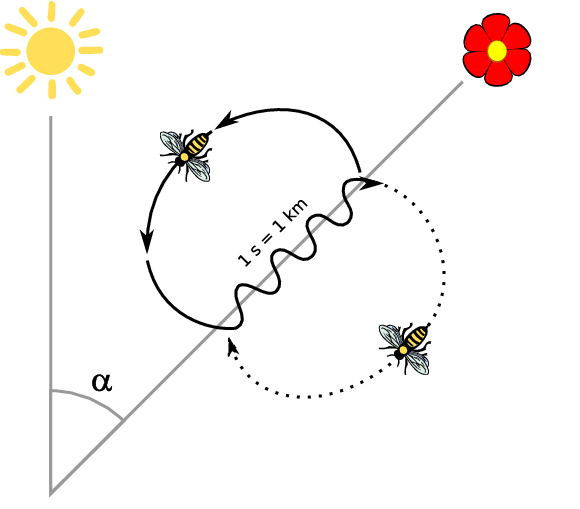
\includegraphics[scale=0.35]{waggle_dance.png}
\end{center}
\caption{Ples pčele koji vrši u košnici, kako bi ukazala drugim pčelama na smer i udaljenost izvora hrane.}
\label{fig:pcela2}
\end{figure}

{\em Udaljenost} izvora se određuje na osnovu krive koju pčela izviđač opisuje prilikom plesa. Ako kruži, izvor se nalazi u radijusu od 50m. Ako je kriva u obliku znaka beskonačno, onda je izvor dalji od 150m; dok je u preostalim slučajevima izvor na udaljenosti između 50m i 150m\cite{plespcela}.

Brzina i vreme trajanja plesa je proporcionalno oceni resursa pčele izviđača. Drugi izviđači takođe mogu opisivati isti izvor nektara. {\em Kvalitet} je veći što je veći broj pčela koje oglašavaju za jedan isti izvor, a samim tim sa njima će poći veći broj sakupljača\cite{bcoalg}. Dokle god se smatraju vrednim, izvori hrane će "reklamirati" pčele sakupljači kroz ples u košnici. Novi regruti mogu takođe učestvovati u plesu i na taj način pozivati što više novih pčela da se priključe sakupljanju. 

\section{Istorija algoritma}
U periodu 1999-2003, srpski akademici - Panta Lučić i Dušan Teodorović, predstavili su osnovne koncepte optimizacije kolonijom pčela kroz sistem pčela {\em(engl. bee system)} dok su vršili istraživanja u {\em Virginia Tech}\cite{algoritam}. Optimizacija kolonijom pčela uvedena je 2005. godine kao metaheuristika za rešavanje problema uparivanja putovanja. Iste godine su Drias i
Yahi modifikovali algoritam optimizacije rojem pčela {\em(engl. bee swarm optimization)} za
problem MAX-W-SAT {\em(engl. maximum weighted satisfiability problem)}. Takođe, D. T. Pham uvodi pčelinji algoritam {\em(engl. bees algorithm)} koji kombinuje
pretraživanje susedstva i nasumično pretraživanje\cite{istorijat}. Dok računarski inženjer D. Karaboga uvodi algoritam veštačke kolonije pčela {\em(engl. artificial bee colony, ABC)} prvenstveno
namenjen numeričkoj optimizaciji.


\section{Pčelinji algoritam}
Pčelinji algoritam je metod pretrage koji oponaša kolonije pčela prilikom potrage za hranom\cite{sajt_algoritma}. Profesor D. T. Pham, zajedno sa svojim saradnicima, je napravio i opisao algoritam 2005. godine.

\begin{figure}[h!]
\begin{center}
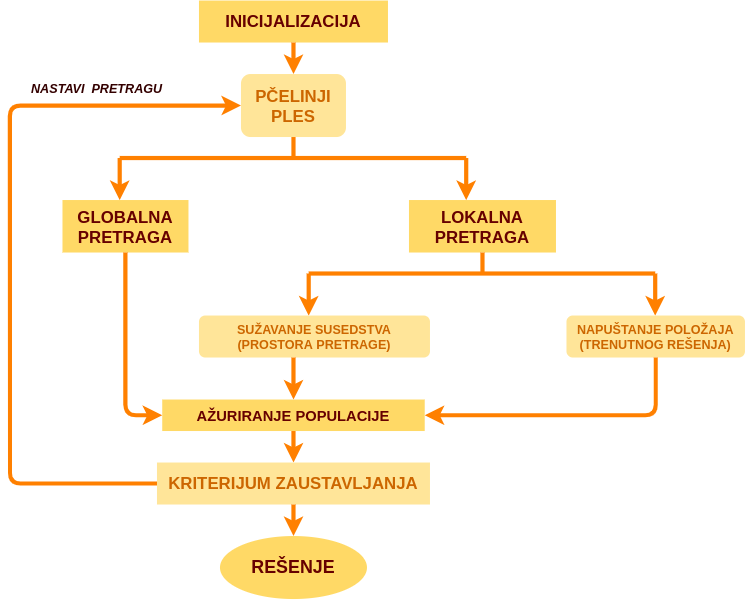
\includegraphics[scale=0.29]{dijagram.png}
\end{center}
\caption{Dijagram sa koracima opšteg pčelinjeg algoritma.}
\label{fig:dij}
\end{figure}
U svojoj osnovnoj verziji izvršava pretraživanje susedstva u kombinaciji sa globalnim pretraživanjem, i može se upotrebiti i za kombinatornu i za kontinuiranu optimizaciju. Koristi populaciju ageansa, odnosno veštačkih pčela, kako bi uzorkovao prostor rešenja\cite{bcoalg}. Pčele izviđači nasumično traže regione visoke funkcije prilagođenosti (globalna pretraga). Najuspešniji izviđači regrutuju promenljiv broj pčela koje tragaju za hranom kako bi pretraživali u okolini najboljih rešenja (lokalna pretraga).
Ciklusi globalne i lokalne pretrage ponavljaju se dok se ne otkrije prihvatljivo rešenje ili ne prođe određeni broj iteracija. Efikasnost ovog algoritma se pokazala u mnogim istraživanjima. 
Među najpoznatijim pčelinjim algoritmima, za optimizacione probleme, nalazi se \textbf{BCO}.
Osnovni koraci dati su dijagramom na slici \ref{fig:dij}.

\subsection{BCO algoritam}
\label{subsec:bco}
Optimizacija rojem pčela je zasnovana na analogiji između prirodnog ponašanja pčela u potrazi za nektarom i ponašanja optimizacionih algoritama u potrazi za optimumom\cite{bcoalg}. Ova metaheuristika je zasnovana na pretraživanju populacije. 
Postoje 2 osnovna pristupa BCO algoritma:
\begin{itemize}\itemindent20pt%
\setlength{\labelsep}{10pt}
	\item \textbf{Konstruktivni BCO} - zasnovan na koracima izgradnje, gde pčele grade rešenje korak po korak
	\item \textbf{BCOi} - zasnovan na poboljšanju celovitih rešenja kako bi se dobila što bolja konačna rešenja \cite{bcoalg}
\end{itemize}

Potrebno je napraviti koloniju veštačkih pčela koje bi tražile dobra rešenja problema u prostoru pretrage. Kako bi kvalitet dobijenih rešenja bio bolji, pčele sarađuju i razmenjuju informacije. Na ovaj način pčele su skoncentrisane na rešenja koja više obećavaju, te postepeno generišu i poboljšavaju pronađena rešenja (sve dok nije postignut zadati kriterijum zaustavljanja).
Opšti algoritam dat je u nastavku:

\begin{lstlisting}[caption={Pseudokod {\em BCO} algoritma \cite{algoritam} },frame=single, label=simple]
// B - broj pcela ukljucenih u pretragu
// N - broj letova od kosnice do cveta i nazad 
	     u jednoj BCO iteraciji
// Inicijalizacija: Dodeljuju se vrednosti promenljivama B i N, 
		 		         odredjuje se kriterijum zaustavljanja
Radi:
    (1) Dodeli prazno resenje svakoj pceli
    (2) Za svako k od 0 do N:
    		// let unapred
    		(a) Za svako i od 0 do B:
    			    Za svako j od 0 do f(N):
    					 (i)  Proceni sve mogucnosti
    					 (ii) Izaberi naredni korak koristeci pravila 
    					      ruleta
    		
    		// let unazad
    		(b) Za svako i od 0 do B:
    			    Proceni kvalitet (parcijalnog/celokupnog) 
    			    resenja	za trenutnu pcelu
    		(c) Za svako i od 0 do B:  
    		    	Odrediti lojalnost na osnovu pravila ruleta
    		    	trenutne pcele i
		    (d) Za svako i od 0 do B:
		       		Ako pceli nije dodeljeno resenje, 
		       		pravilom ruleta izaberi resenje
    (3) Uporedi sva resenja i izaberi najbolje
        Azuriraj x_best i f(x_best) dok kriterijum zaustavljanja
        ne bude zadovoljen
    
dok god (nije zadovoljen kriterijum)
\end{lstlisting}

Populacija se sastoji od {\em B} veštačkih pčela. Svaka od njih zadužena je za proizvodnju jednog rešenja. Različite putanje koje pčele prelaze predstavljaju različita rešenja. Algoritam ima dve faze - \textbf{let unapred} i \textbf{let unazad}. Navedene faze dešavaju se naizmenično\cite{algoritam}.

Kod leta unapred, pčele pretražuju prostor pretrage. Postoji unapred definisani broj koraka koji izgrađuju i/ili poboljšavaju rešenje, koje onda postaje bolje rešenje. Zatim se započinje se s letom unazad.

Kod leta unazad, svaka pčela deli informaciju o kvalitetu svog parcijalnog/celokupnog rešenja. Do optimalnog rešenja dolazi se izračunavanjem funkcije cilja za svako parcijalno/celokupno rešenje, što je analogno plesu pčela u prirodi. Nakon što su rešenja evaluirana, svaka pčela odlučuje (s određenom verovatnoćom) da li će ostati pri svom rešenju ili ne. Pčele koje su pronašle bolja rešenja imaju veće šanse da ih zadrže i reklamiraju. Za razliku od pčela u prirodi, u algoritmu - druge pčele će razmatrati rešenja kao potencijalno dobra, onih pčela koje su ostale verne svojim rešenjima. Kad god neka pčela odbaci svoje rešenje, mora da izabere jedno od reklamiranih rešenja. Pčela donosi odluku sa određenom verovatnoćom - tako da bolja rešenja imaju veće šanse da budu izabrana za naredne korake. Na ovaj način, pri svakom letu unazad, sve pčele se dele u dve grupe. Prvu grupu čine pčele regruteri {\em R}, a drugu neopredeljene pčele {\em B - R}. Vrednosti broja regrutera i neopredeljenih pčela se menjanju od iteracije do iteracije (jednog leta unazad do drugog leta unazad)\cite{bcoalg}. 

U narednom letu unapred, prema konstruktivnom BCO-u, svaka pčela dodaje novu komponentu na pre generisano delimično rešenje. Kod BCOi-a pčele menjaju delove celokupnog rešenja kako bi se postigla rešenja što većeg kvaliteta\cite{bcoalg}.

Faze leta unapred i leta unazad se smenjuju {\em N} puta, dok svaka pčela ne izgradi sopstveno rešenje ili ne uradi izmenu rešenja. {\em N} predstavlja parametar koji služi za definisanje učestalosti komunikacije između pčela. Kada se izvrši {\em N} iteracija/koraka, određuje se najbolje rešenje od svih mogućih {\em B} rešenja. To rešenje se posle koristi pri ažuriranju globalno najboljeg rešenja. Ovime je iteracija algoritma gotova i brišu se svih {\em B} rešenja, te započinje nova iteracija\cite{bcoalg}.

Sve dok kriterijum zaustavljanja nije ispunjen, vrše se iteracije. Mogući kriterijumi zaustavljanja mogu biti maksimalan/zadati broj iteracija ili maksimalan broj iteracija bez poboljšanja funkcije cilja.
Najbolje pronađeno rešenje se daje kao konačno. To rešenje i globalno rešenje.

\subsubsection{Lojalnost pčele}
\label{subsubsec:lojalnost}

Nakon završetka leta unapred, svaka pčela odlučuje da li će ostati verna prethodno pronađenom rešenju ili ne. Ova odluka zavisi od trenutnog kvaliteta rešenja pčele u odnosu na rešenja ostalih pčela. Verovatnoća da je pčela {\em i} lojalna svom prethodnom parcijalnom/celokupnom rešenju, na početku novog leta unapred, opisana je formulom:\\

{\centerline{$p_i^{u+1}=e^{-\frac{O_{max}-O_i}{u}}$} \hfill (*)}\\                             
\begin{itemize}
\item$O_i$ - normalizovana vrednost funkcije parcijalnog/celokupnog rešenja
\item $O_{max}$ - maksimalna vrednost svih normalizovanih
\item u - brojač letova unapred (1, 2, ..., N)
\end{itemize}

     U zavisnosti da li nam treba minimalna ili maksimalna funkcija, normalizacija 
se izvodi na sledeći način:
\begin{itemize}
\item$O_i=\frac{C_{max}-C_i}{C_{max}-C_{min}}$ za minimizaciju
\item$O_i=\frac{C_i-C_{max}}{C_{max}-C_{min}}$ za maksimizaciju
\end{itemize}
gde $C_i$ označava ciljnu vrednost funkcije i-tog pčelinjeg rešenja. \\

Lojalnost pčele zavisi od formule (*), kao i generatora slučajnih brojeva. Ako je slučajni broj manji od izračunate vrednosti, pčela ostaje pri svom rešenju. U suprotnom, neopredeljena je\cite{algoritam}.


\subsubsection{Regrutacija}
\label{subsubsec:regrutacija}

Za svaku neopredeljenu pčelu, treba odrediti kog regruta će slediti. Pritom, uzima u obzir kvalitet reklamiranih rešenja. Verovatnoća da će i-to parcijalno/celokupno rešenje izabrati neopredeljene pčele je: \\

\centerline{$p_i = \frac{Q_i}{\sum_{k=1}^{R}(Q_k)},	    i = 1, 2, . . . R$}

Gde je {\em $Q_k$} normalizovana vrednost funkcije cilja k-tog reklamiranog rešenja. {\em R} je broj regrutera. Svaka neopredeljena pčela se pridružuje jednom od regrutera preko ruleta\cite{bcoalg}.


\section{Primene algoritma}
Ovaj algoritam našao je mnoge primene u inžinjerstvu: optimizacija klaster sistema, manufaktura, upravljanje, bioinžinjering, mnogi problemi optimizacije itd.
U narednoj tabeli su nabrojani problemi koje su naučnici rešavali pomoću optimizacije kolonijom pčela.

\begin{center}
Tabela 1: Primene BCO algoritma od 2001. do 2009. godine
\begin{tabular}{|p{1cm}|p{3cm}|p{5cm}|}
 \hline
Godina & Autori & Primena \\ \hline
2001, 2002, 2003&Lučić i Teodorović&Problem trgovačkog putnika\\ \hline
2003&Lučić i Teodorović&Problem sa usmeravanjem vozila u slučaju nesigurne potražnje\\ \hline
2005&Teodorović i Dell’ Orco&Problem deljenja vozila\\ \hline
2006&Teodorović, Lučić, Marković, Dell’ Orco & Problem trgovačkog putnika i problemi sa usmeravanjem mreža\\ \hline
2007&Marković, Teodorović i Aćimović-Raspopović & Usmeravanje i dodela talasne dužine svim optičkim mrežama\\ \hline
2007& Teodorović i Šelmić & Problem p-medijane\\ \hline
2008& Teodorović & Poređenje performansi BCO algoritma sa performansama drugih algoritama zasnovanih na inteligenciji roja\\ \hline
2009& Davidović, Teodorović i Šelmić & Statičko zakazivanje nezavisnih zadataka kod homogenih višeprocesorskih sistema\\ \hline
\end{tabular}\par
\bigskip
\end{center}

\subsection{Problem trgovačkog putnika}
\label{subsec:prvaprimena}
U postavci ovog problema dato je {\em n} gradova i potrebno ih je sve obići, tako da ni u koji grad ne dođemo dva puta, a da dužina ukupnog puta bude što manja. Lučić i Teodorović su ovo pokušali da reše koristeći metod optimizacije kolonijom pčela. Oni su testirali optimizaciju na velikom broju dobro poznatih testova za testiranje performansi {\em (engl. test benches)} kao što su {\em Eil51, Berlin52, St70} itd\cite{test}. Algoritam je izvršavan na IBM-ovom računaru sa PIII procesorom (533MHz). Rezultati testiranja su prikazani u sledećoj tabeli: 

\begin{center}
Tabela 2: Vrednosti dobijene primenom algoritma \cite{test} 
\begin{tabular}{|p{1.2cm}|p{2cm}|p{2cm}|p{1.4cm}|p{1cm}|}
 \hline
Test & Optimalna vrednost(O) & Najbolja postignuta vrednost pomoću BCO algoritma(B)& (B-O)/O (\%) &CPU (s) \\ \hline
Eil51&428.87&{\textbf{428.87}}&0&29\\ \hline
Berlin52&7544.366&{\textbf{7544.366}}&0&0\\ \hline
St70&677.11&{\textbf{677.11}}&0&7\\ \hline
Pr76&108159&{\textbf{108159}}&0&2\\ \hline
Kroa100&21285.4&{\textbf{21285.4}}&0&10\\ \hline
Eil101&640.21&{\textbf{640.21}}&0&61\\ \hline
Tsp225&3859&3899.9&1.06\%&11651\\ \hline
A280&2586.77&2608.33&0.83\%&6270\\ \hline
Pcb442&50783.55&51366.04&1.15\%&4384\\ \hline
Prl1002&259066.6&267340.7&3.19\%&28101\\ \hline
\end{tabular}\par
\bigskip

\end{center}
Iz tabele može se videti da su najbolje vrednosti, dobijene BCO algoritmom, približne optimalnim vrednostima, kao i da je vreme rada procesora malo. Stoga, može se zaključiti da je BCO dao kvaltetne rezultate.

\subsection{Problem deljenja vozila}
\label{subsec:drugaprimena}
Današnji saobraćaj je veoma zagušen zbog neprestane gradnje novih puteva i novih račvanja. To doprinosi većem broju kašnjenja, dužem putovanju, velikom broju zaustavljanja i povećanju zagađenosti vazduha u gradovima. Zato je bitno pametno iskoristiti postojeće puteve. 

Deljenje vožnje {\em(engl. ride-sharing)} je jedna od korišćenijih TDM {\em (engl. Travel Demand Management)} tehnika. U okviru ovog koncepta dve ili više osoba dele isto vozilo kako bi stigli do svojih destinacija. Prevoznik mora da poseduje sledeće informacije kako bi dobro isplanirao put:
\begin{itemize}\itemindent20pt%
\setlength{\labelsep}{10pt}
       \item kapacitet vozila (broj ljudi u vozilu)
       \item mesto odakle se kreće za svaki dan u nedelji
       \item krajnja destinacija za svaki dan u nedelji
       \item vreme željenog polaska i/ili dolaska za svaki dan u nedelji
       \item dani u nedelji, kada je osoba spremna da učestvuje u deljenju vozila 
\end{itemize}

Teodorović i Dell’ Orco želeli su da osmisle rutu i raspored vozila i putnika za celu nedelju, tako da ukupna dužina putovanja za sve učesnike bude minimalna. Razvili su model koji se oslanja na BCO.
Ovaj model testiran je na uzorku vozila koja su kretali iz malog grada u Italiji - Trane, do mesta Bari. Učestvovalo je 97 putnika. Kapacitet svakog vozila bio je 4 putnika.

U ovom slučaju, algoritam je odredio da 96 (= 24*4) od 97 putnika daju najbolju putanju. Ne postoji standardni metod u literaturi za određivanje najbolje metode za optimalno deljenje vožnje. Ovo je bio samo pokušaj da se razvije metodologija koja bi mogla da reši ovaj problem\cite{voznja}.

\section{Zaključak}
\label{sec:zakljucak}
U ovom radu predstavljena je optimizacija kolonijom pčela, metaheuristička metoda inspirisana ponašanjem pčela i najmlađa tehnika koja koristi inteligenciju roja. Bavili smo se komunikacijom između pčela i međusobnoj podeli posla u košnici. Posebna pažnja posvećena je samom algoritmu, koji se uz određene modifikacije može prilagoditi za različite probleme optimizacije u upravljanju, inženjeringu ili kontroli. Takođe, ukratko je opisana primena na problem trgovačkog putnika i problem deljenja vozila, sa kojim se svakodnevno susrećemo. BCO ima mogućnost da putem razmene informacija i regrutovanja intenzivnije vrši pretragu u onim regionima prostora rešenja koji više obećavaju. Ipak, nije široko korišćen za rešavanje stvarnih problema.

Zanimljivi aspekti budućeg istraživanja mogu biti homogenost pčela, različiti mehanizmi razmene informacija i različiti mehanizmi saradnje. Takođe, jedna od interesantnih praktičnih primena mogla bi da bude i primena pčelinjeg algoritma na naše elektronske uređaje. Naime, svima nam je dobro poznata situacija u kojoj se mobilni telefon, laptop ili neki drugi uređaj zagrejao ili prestao sa radom usled velikog korišćenja. O rešavanju ovog problema, inspirisan prirodom (tačnije pčelama), govori Ali Abuassal u svom doktorskom radu (za znatiželjne, link ka ovom radu dat je u dodatku).

\newpage
\addcontentsline{toc}{section}{Literatura}
\appendix
\bibliography{seminarski} 
\bibliographystyle{plain}

\appendix
\section{Dodatak}
Za one koji žele da znaju više, doktorski rad Ali Abuassala možete pronaći na:
\url{https://pure.york.ac.uk/portal/en/publications/artificial-bee-colonyinspired-runtime-task-management-for-manycore-systems(83f1aad7-3e26-4609-b0df-03af36d0d330).html}.

\end{document}
